\chapter{Elba The Car}

%Introduction
\section{Introduction}
Elba is the name of one of the two cars of the Eco Cars project housed by
ITRL\@.  Elba is an Urban Concept Vehicle (UCV) and have been a continuous
project ongoing for many years. The design and propulsion system, along with the
name of the UCV of Eco Cars have changed over the years and Elba is the name of
the current active car. In difference to a couple of years ago when Elba was
purely driven by an electric motor, Elba is today propelled by a parallel
electric-ethanol hybrid. The platform has been continuously improved and altered
to become the complex hybrid that exist today. The goal of Elba is to
participate in the Shell Eco-marathon.

\subsection{Propulsion}
Elba combines two electrical
motors and one internal combustion engine (ICE). The electrical motors are one
200 W direct current (DC) motor connected directly to the drive shaft and one
1.1 kW brushless DC motor (BLDC) connected via the clutch to the drive shaft.
The one-cylinder four-stroke ethanol powered ICE is connected to the drive
shaft via the clutch. These three provide a driving torque to the rear drive
shaft. The drive shaft is then connected to the right rear wheel via an 1:10
ratio planetary gear. The car fits a single human and he or she is also the
driver. The driver steers the car manually and decides upon a reference speed
that the car should follow and has the option to decide what motor/engine
combination that should be used at a specific time.

\subsection{State at start of project}
The car was in working condition when the project started, but had several
problems, including that the clutch was slow and unreliable, the overall power
output might not have been enough to be efficient on the new track, none of the
potential drivers would fit in the driver compartment and the horn disturbed the
entire electrical system.  These issues where, together with the competition
rules, the primary base for the decisions that where taken and related to the
car. Some of the work done to correct these problems where a matter of reshaping
some metal piece and bolting it back in the car so that the driver could reach
the brakes, while other required an entire team of people to get a new, working,
ethanol engine in the car.

%System Overview
\section{System Overview}
\subsection{Electronic Control Units}
The car has four electronic control units (ECUs) that are responsible for
controlling different parts of the car. An overview of the communication between
the ECUs can be seen in Figure~\ref{fig:communication_overview}

\begin{figure}[H]
    \centering
    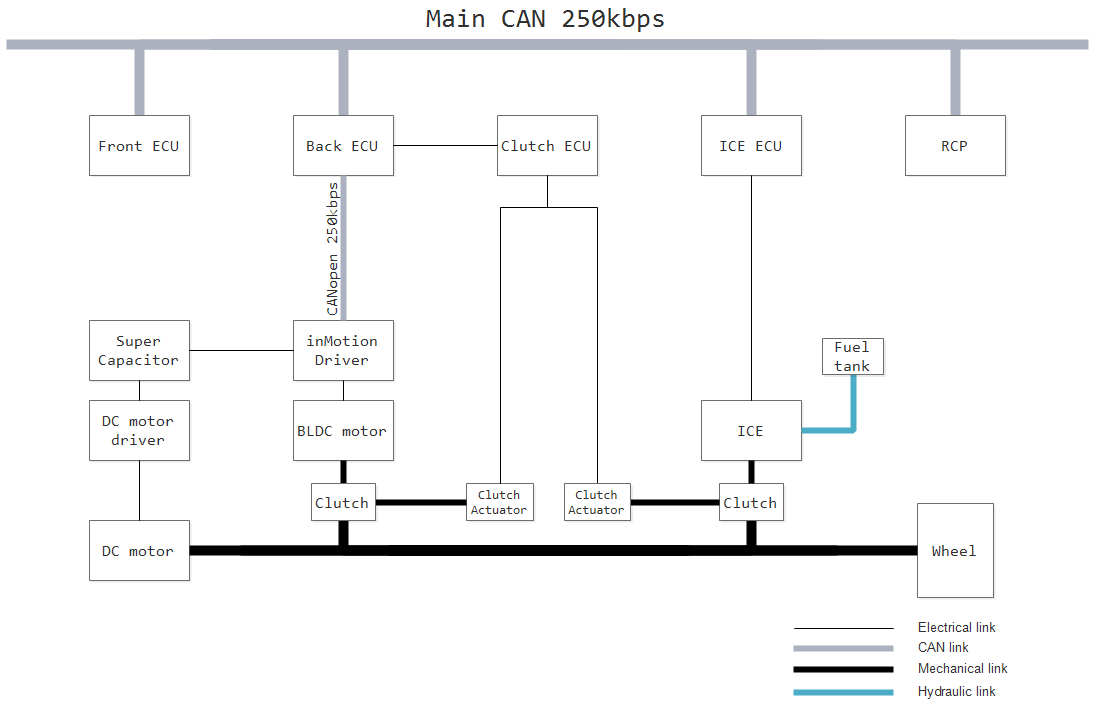
\includegraphics[width=1\textwidth]{./img/elba_communication_overview}
    \caption{Overview of the communication system and drivetrain in
    Elba}\label{fig:communication_overview}
\end{figure}

\noindent
The Front ECU is responsible for the human user interface, which is the buttons where the
driver is able to decide drive mode and reference speed if the car is in manual
mode. It transmits speed and drive mode on the CAN bus.\\
The Back ECU controls the two motors via separate motor controllers. It has
veto over the ICE and Clutch.\\
The internal combustion engine is controlled by the ICE ECU and this is its sole
purpose, it does nothing else. It reads the lambda sensor and motor
temperature sensors to control the fuel injection.\\
The Clutch ECU controls the clutch, and it interfaces to two H-bridges which in turn
steers the linear actuators.  

\subsection{Communication}
The car uses a CAN network to communicate between the distributed
micro-controllers. Any data that is needed elsewhere is sent on the CAN-bus.
Each CAN message consists of a CAN id, a 32 bit upper data integer and a 32 bit
lower data integer. 

Messages sent from Front ECU are sent with id 170, from Back
ECU with id 169 and 113, and from ICE ECU with id 114. GPS data from the
data-logger/GPS-unit Race Capture Pro are sent with id 180. Data position in the
messages on the CAN-bus can be seen in table~\ref{table:CAN}, counting the
least significant bit as bit 1. The lower data accounts for bit
position 1--32 and upper data 33--64.
\begin{table}[H]
    \caption{Data position in different CAN messages on the CAN
    bus.}\label{table:CAN}
    \begin{center}
        \begin{tabular}{lcl}
            \textbf{Data} & \textbf{Id} & \textbf{Bits}\\
            \toprule
            Reference Speed & 170 & 1--16 \\
            Brake & 170 & 17 \\
            Reference Mode & 170 & 20--23 \\
            Auto & 170 & 24 \\
            Current Speed & 169 & 1--16 \\
            Supercapacitor Voltage & 169 & 17--32 \\ 
            Current Mode & 169 & 33--36 \\ 
            BLDC motor current & 169 & 37--48 \\
            Distance & 169 & 49--64 \\
            ICE RPM & 114 & 1--16 \\
            ICE on/off & 113 & 1--2 \\
            Fuel injection time & 114 & 17--32 \\
            GPS longitude & 180 & 1--32 \\ 
            GPS latitude & 180 & 33--64 \\
            \bottomrule
        \end{tabular}
    \end{center}
\end{table}
Another CAN network is used between the Back-ECU and the inMotion driver that
controls the BLDC motor. This network uses the protocol CANopen that
lies on top of the CAN bus. The instrumentation panel communicates via Bluetooth
with the Race Capture Pro 2 (RCP2).

\subsection{Energy supply}
All energy used to propel the car forwards (during the competition) comes from
the ethanol fuel, but electrical energy can be stored in the super-capacitor.
When the electrical motors generate energy it can be stored in this
super-capacitor for later use. The car can only start from standstill using one
of the electrical motors with energy from the super-capacitor.  

%Software and Simulation
\section{Software and Simulation Models}
Using Model Based Development (MBD), relies on verified systems models on various
levels. Elba benefits form a full system model to simulate fuel efficiency and
each ECU have a corresponding Simulink model from which all code is compiled.

\subsection{Plant Model}
The Simulink plant model is supposed to be a full system model capable of
estimating fuel consumption over an entire SEM attempt. When any component,
which has an effect on propulsion, is changed on the car the plant model must
also be updated. Naturally the goal with MBD is that any change can be simulated
with the plant model, approved and then the car is updated. But not all
simulations can be done beforehand, which was the case for the new ICE\@. 

The plant model is functionally very similar to the old model described
in~\cite{elba2015}. The structure of the model was improved to give a clearer
view, a way of including the track profile was added and errors in some models
were corrected. Also, the work of~\citep{liu2016} was included in the form of a
reference speed lookup table. The plant model also includes a model of the
testrig to simulate forces and torques it is required to output.

Since the new ICE couldn't be properly mapped, the plant model uses parameters
from the old ICE\@. This needs to be considered when interpreting results from
simulations on the plant model.

\subsection{ECU software}
All ECUs use Arduino (Due or Mega) micro-controllers, which Simulink has
compiler support for. This means that Simulink models can be compiled and
uploaded to the Arduino directly from Simulink. The Simulink to Arduino coupling
also gives the option of running ``external mode'' a Hardware in the loop type
compile mode.  This makes it possible to look at values and signals, running on
the ECU, in real-time.

%Data logging
\section{Data logging} 
The need for collecting data is a very important aspect when
it comes to iteration during the development of the car. In order to determine
if changes make the car perform and handle better there is a real need for
comparing data. In Elbas case, logging data from multiple ECU's is a must in
order to have a complete picture of the car. The absolute best way to log all
the relevant data is to log the CAN-bus. All the information sent on CAN is
relevant and of highest interest. There was always the possibility of having the
laptop in the car while driving but this didn't seem to be the best way. After
experimenting with different solutions, including making our own logging device,
was the Race Capture Pro 2 (RCP2) found to meet the requirements,
see Appendix~\ref{app:RCP}. It has the possibility to communicate with two CAN-channels
and logging different custom identifiers as virtual channels. With it's eight
analogue input channels and three digital I/O channels it is also very suitable
for logging both analogue and digital signals, which is a really good addition.

\subsection{RaceCapture Pro 2}
The RCP2 is a customizable lap timer, data logger and telemetry system designed
for racing cars. The RCP2 comes with a software GUI that is used for
configuration and this software also holds the interface for scripting
configurations.  The language used in the RCP2 is Lua and this can used to
configure everything in the RCP2. One of the two CAN channels of the RCP2 is
connected to the main CAN-bus of Elba, as can be seen in
Figure~\ref{fig:communication_overview}.  The main purpose of the RCP2 is to log
data, both data communicated on the CAN bus and the GPS-position from the dongle that
was provided. To be able to log the custom CAN-bus, there is a function called
virtual channels, this allows for customized CAN id's to be logged. There is
currently three different virtual channels that have been set up lo log messages
sent from the back, front and ICE ECU\@. These three virtual channels is logging
messages with ID 114, 169 and 170, and what is sent with these messages can be
seen in Table~\ref{table:CAN}.
Besides the logging function, the RCP2 is used to track Elbas position on the
track. This is done by a GPS-dongle that was provided with the RCP2 and have the
following specifications,
\begin{align}
   CEP&=2.5\textnormal{m}\\
   R_{sample}&=50\textnormal{Hz}.
\end{align}
More on how the GPS signal is used to position Elba on the track can be found in
Section~\ref{sec:opt_pos_recon}.\\
The logging file that the RCP2 produces is a Comma Seperated Value file, even
though the file format is not standardized, there is a wide spread when it
comes to log-files, database information, serial data streams etc.
The file format is very convenient for usage with MATLAB, as there are built in
functions to load the CSV file and extracting information can be done with
minimal effort. During the project a MATLAB script have been developed to both
extract the right information and plot the interesting data. The exact way the
RCP2 loggs data can be found at~\cite{RCP2_log} 

%Requirements
\section{Requirements}
\subsection{Rules}
At Shell Eco Marathon all vehicles must pass two inspections before the vehicle
is allowed to enter the track. First a safety inspection evaluating if it's
dangerous to have the vehicle on the track, both for the driver and other
vehicles. And second a technical inspection asserting if the vehicle complies
with the competition rules.

Therefore all rules regarding the car where seen as requirements. These requirements where passed on to the respective subgroups to ensure compliance at all levels. 

%Design Decisions
\section{Design decisions}
\subsection{Clutch decisions}
%1. What the old team told us
%2. What we told MD to do
%3. What MD did
%4. Problems still
%5. Finding the problem
%6. Fixing the arms

One of the major problems with the car have been the clutch.
Figure~\ref{fig:Drivetrain} illustrates the mechanical components of the
drivetrain of Elba.

\begin{figure}[H]
    \centering
    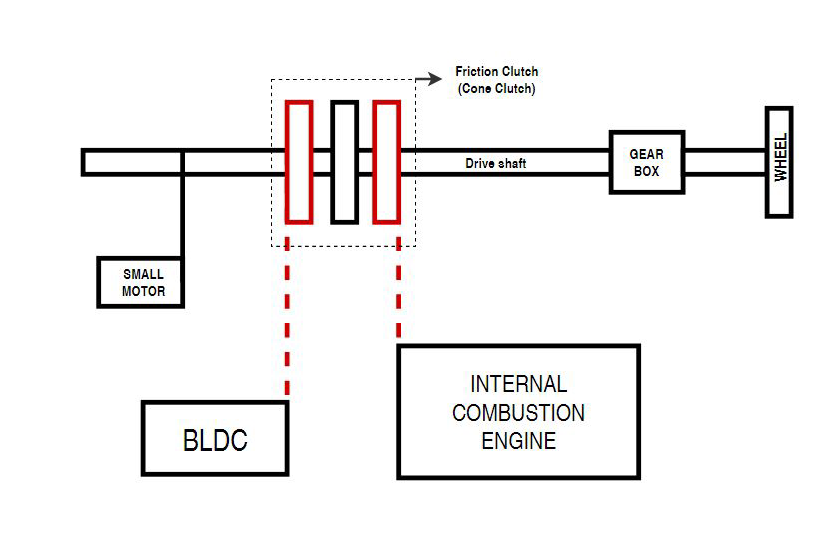
\includegraphics[width=1\textwidth]{./img/Drivetrain}
    \caption{Illustration of the mechanical components of the drive train, where
    the red plates can move towards the center plate to engage and disengage the
    motors to the drive shaft.}\label{fig:Drivetrain}
\end{figure}
At the start of the project, the problem was that the clutch actuators were
oversized and thus giving more force than necessary for the clutch to engage
properly. When the clutch was engaged, there was too much actuator force, and so
the clutch plate on the ICE side got stuck center plate and could not be
disengaged using the actuator.

To solve the mechanical problems it was decided to appoint one team from the
machine design department to work solely on the mechanical parts of the clutch.
The Mechatronics team decided to completely remake the clutch ECU to make it
more robust. Despite the new ECU and the work performed by the machine design
team, which can be read about in Appendix~\cite{MD_report}, there was problems
with the clutch when it was time to race. The problems was of the same
mechanical nature as before the rework, where the clutch plate on the ICE side
could not be disengaged from the drive train. To solve this problem, several
solutions have been investigated. The clutch mechanism has been controlled by
time rather than position. One approach was to use the built in hall sensor in
the actuator to control the position. One other idea was to use an external
current sensor on the clutch ECU to control the position. A third idea was to
continue using time as reference, but increase it so that an end position is
always reached, which can be used as a reference position.

When investigating alternative three, using longer time to engage and
disengage the clutch, a new problem was discovered. It appeared that even though
the clutch was not stuck to the center plate it still could not be properly
disengaged. This was due to the geometry of the lever arm which pushes the
clutch plate.  After this important insight the drive train was disassembled and
new lever arms were constructed and manufactured. When the drive train was
assembled again the clutch worked like expected. Figure~\ref{fig:clutch}
and~\ref{fig:old_clutch} shows both the new and old lever arms.

\begin{figure}[H]
    \centering
    \begin{subfigure}[H]{0.55\textwidth}
    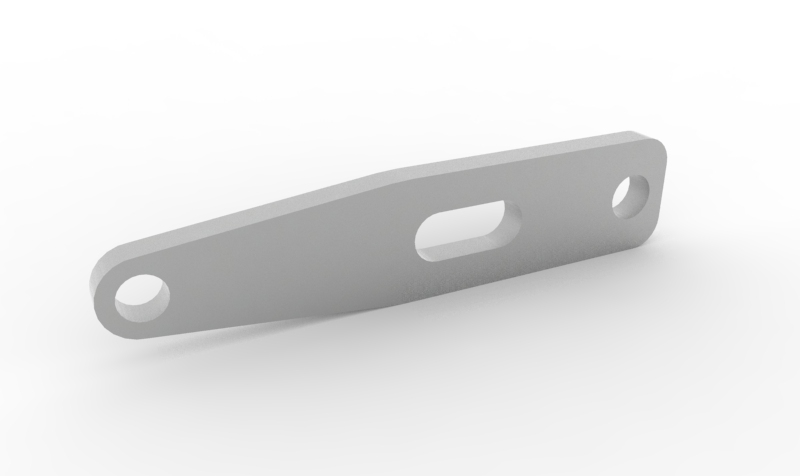
\includegraphics[width=\textwidth]{./img/clutch}
    \caption{The new clutch lever arms}\label{fig:clutch}
    \end{subfigure}
    \begin{subfigure}[H]{0.44\textwidth}
    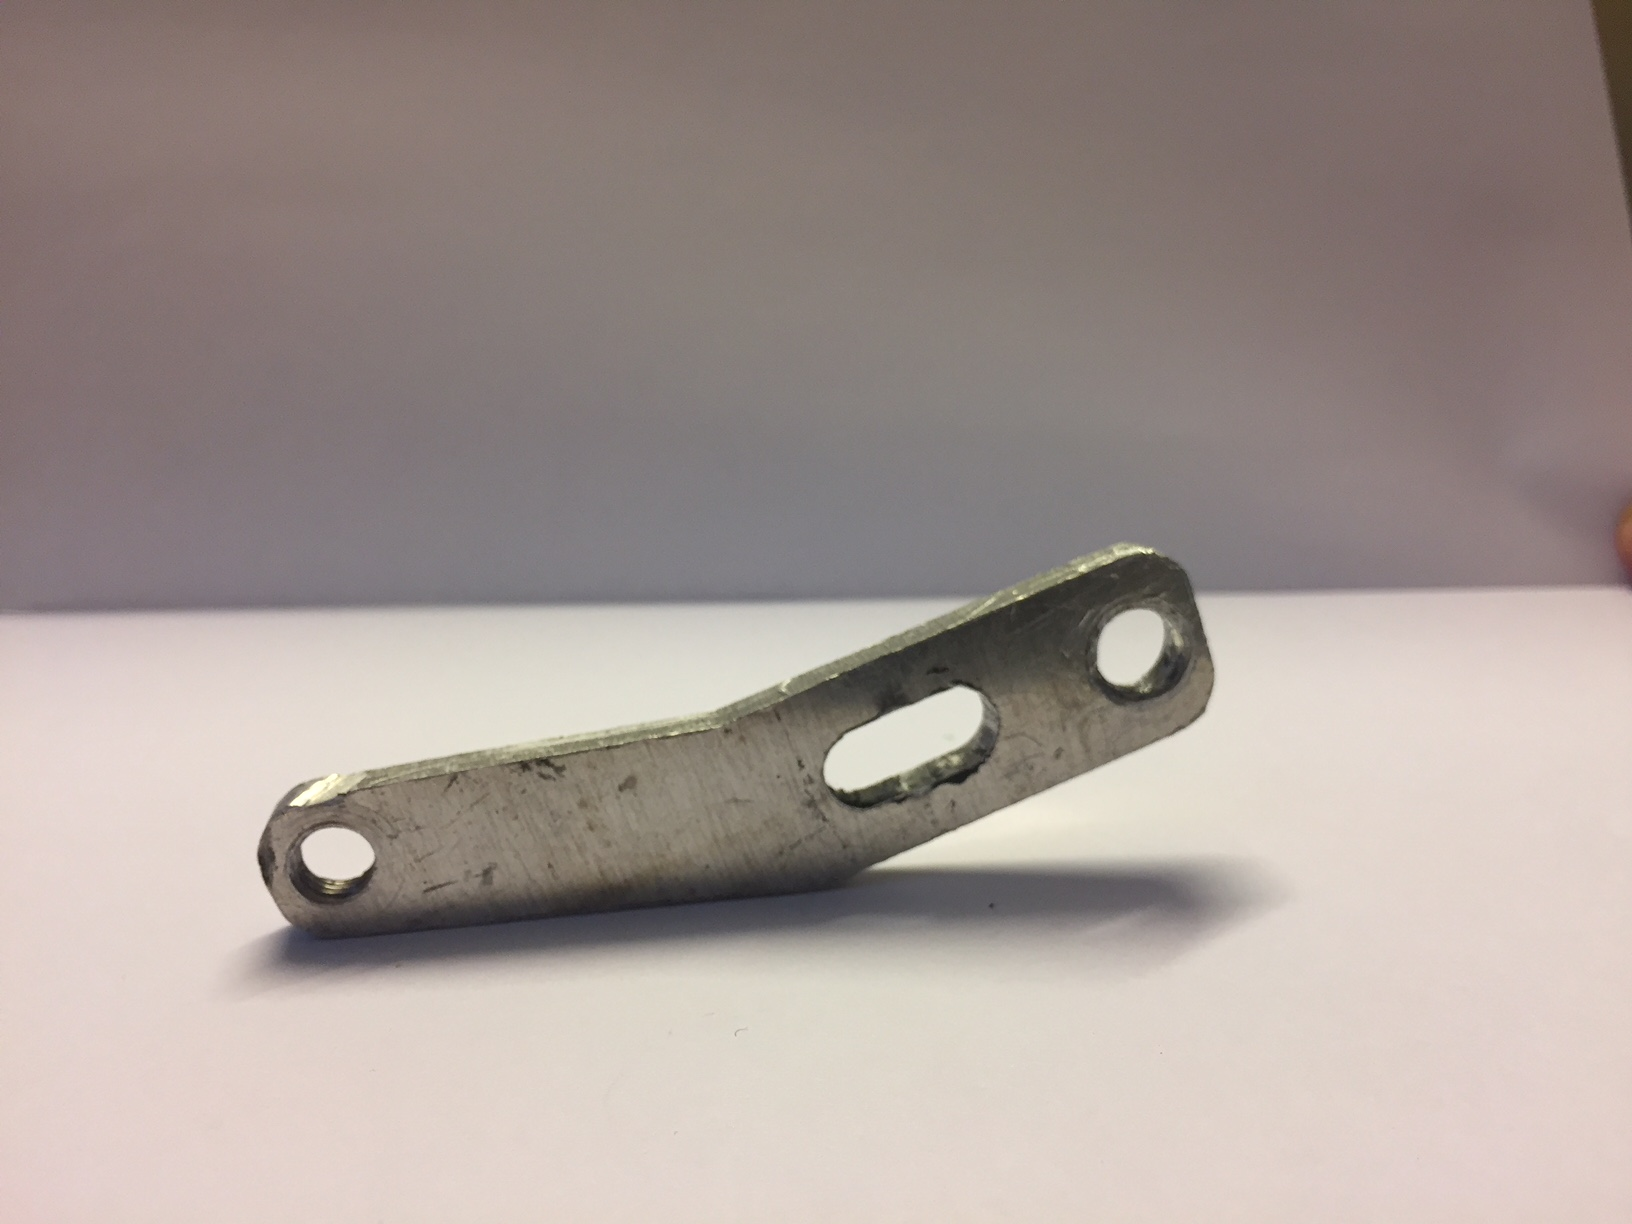
\includegraphics[width=\textwidth]{./img/Clutch_old}
    \caption{The old clutch lever arms}\label{fig:old_clutch}
    \end{subfigure}
    \caption{This image shows the difference between the old and the new lever arms that are used to push the clutch plates.}
\end{figure}

\begin{figure}[H]
    \centering
    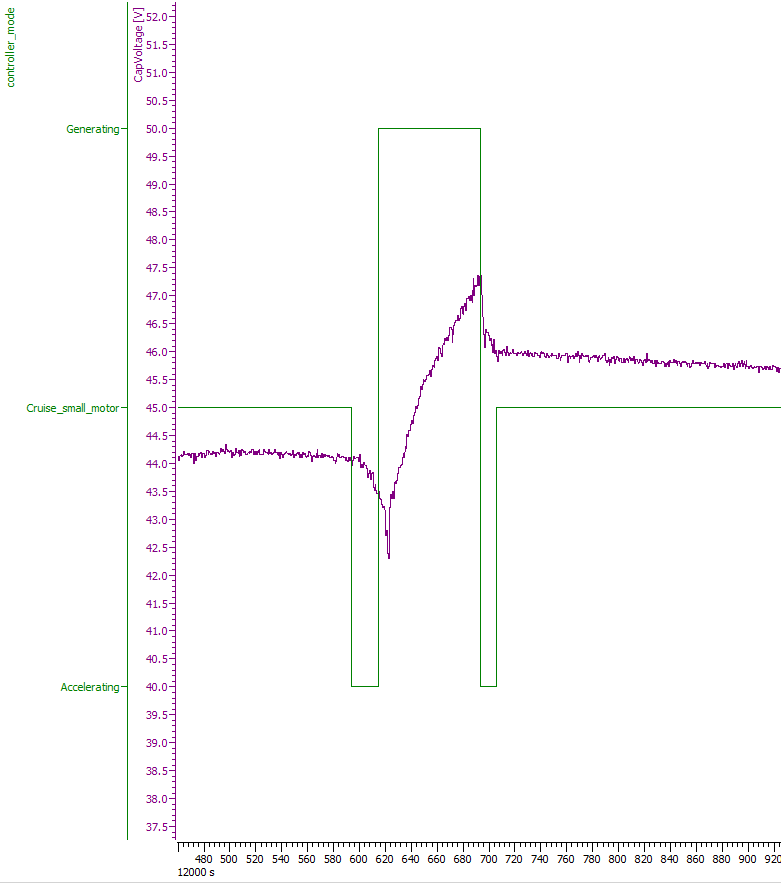
\includegraphics[width=0.75\textwidth]{./img/elba_capvoltage_regen}
    \caption{Capacitor voltage and drivemode as a function of time}\label{fig:elba_capvoltage_regen}
\end{figure}

Figure~\ref{fig:elba_capvoltage_regen} illustrates a sequence from CANoe where the capacitor is charged by changing mode from the small DC motor when the voltage is low and charging to a higher voltage level then changing back to the small DC motor.

\subsection{Internal Combustion Engine and ICE ECU}
One of the requirements from the ICE-department was that the ICE should be run
on ethanol. An engine running on ethanol needs to have a higher compression ratio
than a petrol engine~\cite[p.8]{ICE_report}.
The requirements engineering and modifications on the new ICE was set by the ICE
team based on the requirement given in the rules, along with recommendations from 
previous year. 


It had been said that last years ICE where too powerful, when the car regenerated its
maximum energy at the average track speed the car still wanted to accelerate. 
Going faster than required saves time but is a waste of energy and therefore bad at SEM.
A new ICE was proposed with 50 cc compared to earlier 57 cc. Another major difference 
was that the new motor had an horizontal output shaft compared a vertical one. 
This meant that no bevel gear had to be used, which was a major point of failure earlier.
The ICE had to be shipped relatively fast and a requirement from ICE-group supervisor was that 3 identical engines had to be bought. This limited the choice even further. 
Which motor that was chosen in the end and why is motivated in greater detail in appended paper \citep{ICE_report}.

To control the new engine, a new ICE ECU was needed. It was also decided
that the new ICE ECU would contain more sensor inputs as well as the possibility
to control the ICE ignition. All functionality of the old ICE ECU would still be
present, namely:
\begin{itemize}
    \item Simulink TLC software.
    \item Feedback control loop of injection time.
    \item Lambda value sensing.
    \item Encoder reading with index pulse from ICE\@.
\end{itemize}
More sensor data together with ignition control would give possibilities
for more exact control of the ICE\@. The extra features of the new ECU were:
\begin{itemize}
    \item Motor oil temperature sensing.
    \item Ambient air temperature sensing.
    \item Ignition control.
\end{itemize}
The features were implemented on the ECU PCB and the system was designed so that
the sensors and features could be implemented incrementally according to the
time and need of the project. Given that the amount of time that would be needed
to get the car in working condition before the race was not easily planned
beforehand, it was beneficial to have a base functionality with flexibility to
add features.

\subsection{Door}
The car is required to have a door, with a large enough entrance and working
locking mechanism~\cite{semrules16c1}. Since the old, layered carbon fibre door
was too flimsy and also back hinged (there is a reason its called ``suicide door''),
it was decided a new, sturdier, door would be made. Two lightweight-construction
student took this upon them self as a bachelors project. 

The new door where constructed in a carbon fibre sandwich style and was open in
a scissor manner. The door became sturdier but the hinges where less than ideal
and the closing mechanism did not work.

%Results
\section{Results}

\subsection{Competition}
At the time the team arrived in London the ICE had never been started with only
ethanol as fuel, the door had to be mounted and the team needed to do a number
of small changes to be able to pass both inspections. Most time was spent to get
the engine running, but it was never able to run for more than a couple of
strokes. 

Both the technical inspection and safety inspection were passed. There where a
few complaints: The doors closing mechanism was insufficient, the indicator
lights were to weak, and the fire-extinguishers expirations date had passed.
All these had to be reinspected before Elba was given a pass.

It was decided that one attempt should be made even if the engine never had been
started properly. Since the car must be rolling to start the ICE the inertia of
the car will keep the ICE turning even if it misfires (the wheel inertia is not
enough for this). This meant that the ICE started once the car finally was
running during the attempt. %But it was soon discovered that the engine could
%not be shut off, if the clutch was disengaged the engine kept running and
%revving at dangerous levels. %KOMMENTAR: Känns som att vi kan utelämna denna
%bit... :D /Emil
At the compulsory stop after one lap the clutch to the ICE did not properly
disengage, causing Elba to stall the engine with clutch engaged. While trying to
get going again the clutch could not be disengaged and the attempt had to be
aborted.

Therefore Elba never got a competition result. 

\subsection{End of project}
%%in this section we will write what is done so far and the.

A lot has happened with Elba since the competition in June. At the end of this
project the car is finally in fully working condition. Both the clutch and the
ICE which were the major problems have been fixed to a point where they work
sufficiency, but not optimal. For the ICE it would be needed to study the engine
parameters to make it run more efficiently. The clutch is very slow and would be
much more energy efficient if it could engage and disengage much faster. One way
could be to study the actuator timings and decrease the distance that the
actuator moves, but still keep the proper functionality.
